\documentclass[a4paper,11pt,french]{article}
\usepackage[utf8]{inputenc}

\usepackage[T1]{fontenc}
\usepackage[francais]{babel} 
\usepackage[top=2cm, bottom=2cm, left=2cm, right=2cm, includeheadfoot]{geometry} %pour les marges
\usepackage{lmodern}
\usepackage{pict2e}
\usepackage{fancyhdr} % Required for custom headers
\usepackage{lastpage} % Required to determine the last page for the footer
\usepackage{extramarks} % Required for headers and footers
\usepackage{graphicx} % Required to insert images
\usepackage{tabularx, longtable}
\usepackage{color, colortbl}
\usepackage{lscape}
%\usepackage[hidelinks]{hyperref}
\usepackage{longtable}
\usepackage{multirow}
\usepackage{rotating}
\usepackage{gensymb}

\usepackage{algorithm}
\usepackage{algorithmic}


\linespread{1.1} % Line spacing

% Set up the header and footer
\pagestyle{fancy}
\lhead{\textbf{\hmwkClass -- \hmwkSubject \\ \hmwkTitle \\ \hmwkDocName}} % Top left header
\rhead{
\includegraphics[width=10em]{logo_univ.png}}
\lfoot{\lastxmark} % Bottom left footer
\cfoot{} % Bottom center footer
\rfoot{Page\ \thepage\ / \pageref{LastPage}} % Bottom right footer
\renewcommand\headrulewidth{0.4pt} % Size of the header rule
\renewcommand\footrulewidth{0.4pt} % Size of the footer rule

\setlength{\headheight}{40pt}

\newcommand{\hmwkTitle}{\'Etude sur l'installation/acceptation d'une autorité de certification} % Assignment title
\newcommand{\hmwkClass}{Master 2 SSI } % Course/class
\newcommand{\hmwkAuthorName}{Julien BOURDON} % Your name
\newcommand{\hmwkSubject}{Recherche} % Subject
\newcommand{\hmwkDocName}{} % Document name

\newcommand{\version}{1.0} % Document version
\newcommand{\docDate}{28 novembre 2013} % Document date
\newcommand{\checked}{} % Checker name
\newcommand{\approved}{} % Approver name

\makeatletter
\newcommand{\resettranslate}{\let\translate\@firstofone}
\makeatother

\definecolor{gris}{rgb}{0.95, 0.95, 0.95}

\title{
\vspace{2in}
\textmd{\textbf{\hmwkClass :\ \hmwkTitle}}\\
\normalsize\vspace{0.1in}\small{Due\ on\ \hmwkDueDate}\\
\vspace{0.1in}\large{\textit{\hmwkClassInstructor\ \hmwkClassTime}}
\vspace{3in}
}

\author{\hmwkAuthorName}
\date{} % Insert date here if you want it to appear below your name


\usepackage{amsmath}
\begin{document}
\newcount\startdate
\newcount\daynum
%\pgfcalendardatetojulian{2013-01-021}{\startdate}
\pagestyle{fancy}

\vspace*{5cm}
\begin{center}\textbf{\Huge{\hmwkDocName}}\end{center}
\vspace*{4.5cm}
	

\fcolorbox{black}{gris}{
\begin{minipage}{15cm}
\begin{tabularx}{10cm}{lXl}
	\bfseries{Version} & & \version\\
	& & \\
	\bfseries{Date} & & \docDate\\
	& & \\
	\bfseries{Rédigé par} & & \hmwkAuthorName \\
	& & \\
	\bfseries{Relu par} & & \checked \\
	& & \\
	\bfseries{Approuvé par} & & \approved \\
	& & \\
\end{tabularx}
\end{minipage}
}

\newpage

%Tableau de mises à jour
\vspace*{1cm}
\begin{center}
\textbf{\huge{MISES À JOUR}}\\
\vspace*{3cm}
	\begin{tabularx}{16cm}{|c|c|X|}
	\hline
	\bfseries{Version} & \bfseries{Date} & \bfseries{Modifications réalisées}\\
	\hline
	1.0 & 28/11/2013 & Création\\
	\hline
	& & \\
	\hline
	\end{tabularx}
\end{center}

%La table des matières
\clearpage
\tableofcontents
\clearpage

\section{Objet}

De nos jours, nous avons besoin d'authentifier les sites auxquels on veut accéder pour être sur que les données cruciales que nous manipulons ne tombent pas en de mauvaises mains. Pour ce faire, on utilise des certificats signés par des autorités en qui on peut avoir confiance.
Ces autorités sont répertoriées dans nos machines et plus précisément dans nos navigateurs par le biais de certificats d'autorité.
Nous allons maintenant voir comment on peut faire accepter l'installation d'une nouvelle autorité sur sa machine en quelques clics.


\section{Installation par un administrateur mal intentionné}
Nous prenons, ici, le cas d'un administrateur ayant un accès à tous les ordinateurs d'une entreprise.
Cette personne veut faire accepter une autorité de certification dont il est le propriétaire pour pouvoir lire tous les paquets qui transitent et surtout les chiffrés.
Nous allons expliquer comment faire pour les principaux navigateurs utilisés sous linux.
Voilà un tableau comparatif des pourcentages d'utilisation des navigateurs : 

Moyenne générale (Décembre 2013) :
\begin{itemize}
\item{Chrome} 		34,73\%
\item{Internet Explorer}		 22,89\%
\item{Firefox} 		18,25\%
\item{Safari} 		16,19\%
\item{Opera}	 		1,57\%	
\item{Autres} 		6,38\%
\end{itemize}	

Nous allons donc privilégier Firefox et Chrome.
\newpage
\subsection{Mozilla Firefox}

Tout d'abord, l'administrateur ouvre Firefox puis clique sur Edit > Preferences.

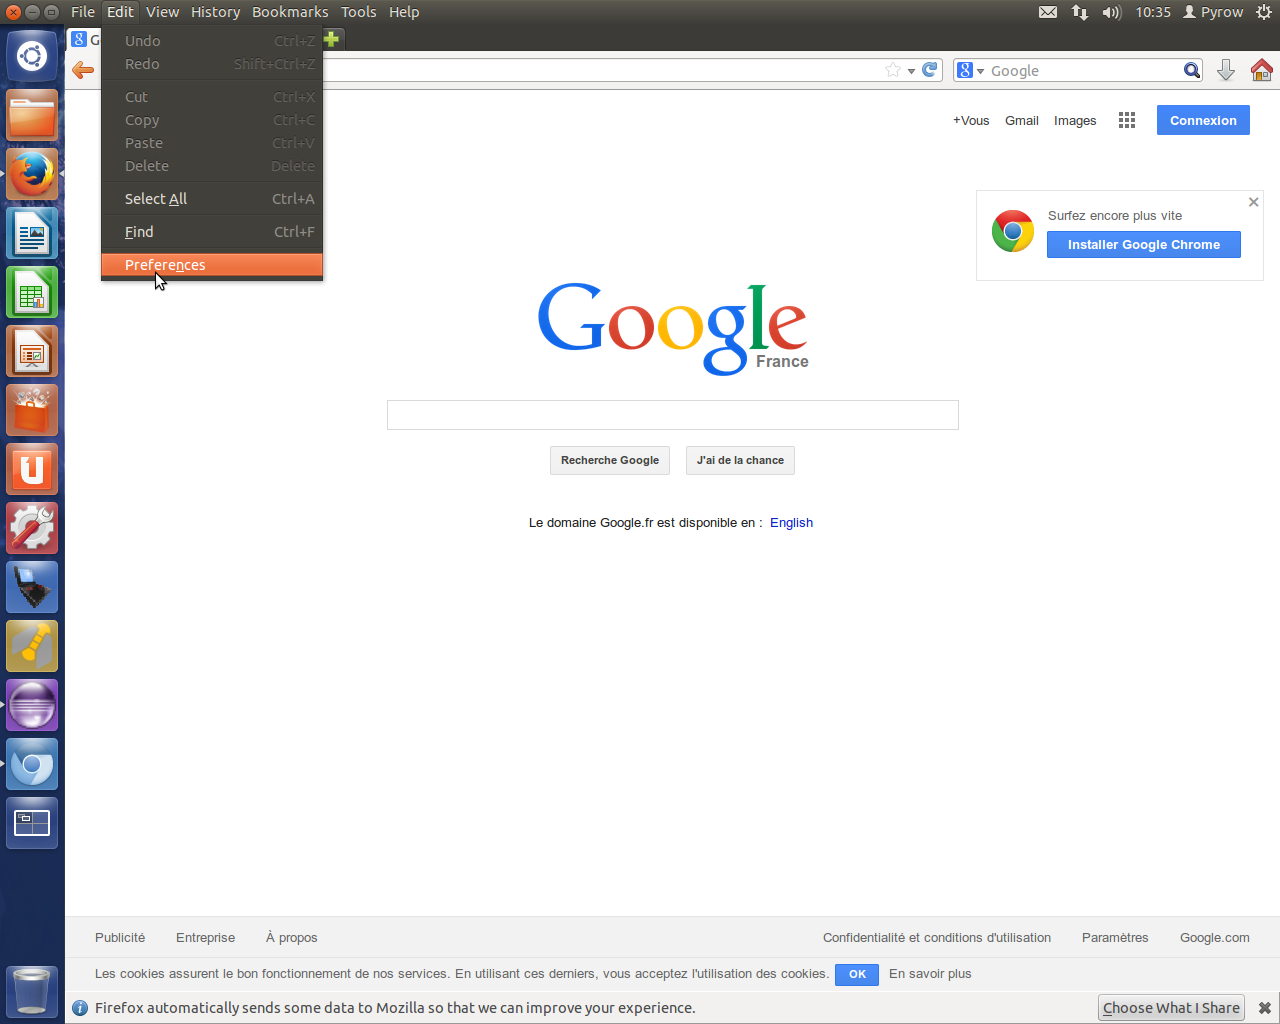
\includegraphics[width=\textwidth]{images/OngletPref.png}
\newpage
Ensuite, il choisit Advanced > Certificates > View Certificates.

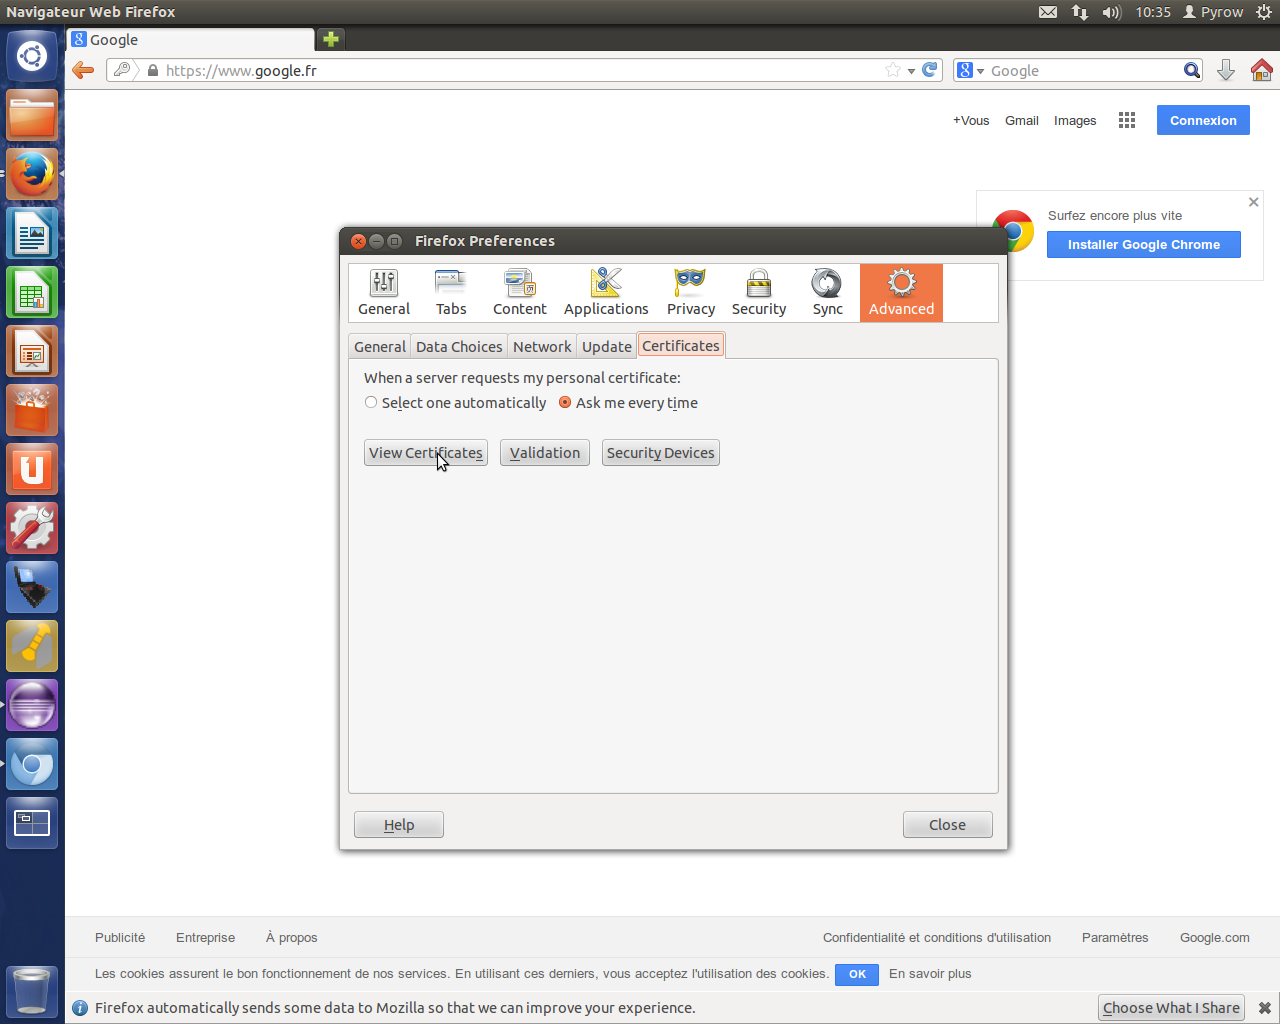
\includegraphics[width=\textwidth]{images/OngletCert.png}
\newpage
Il va ensuite dans Authorities > Import.

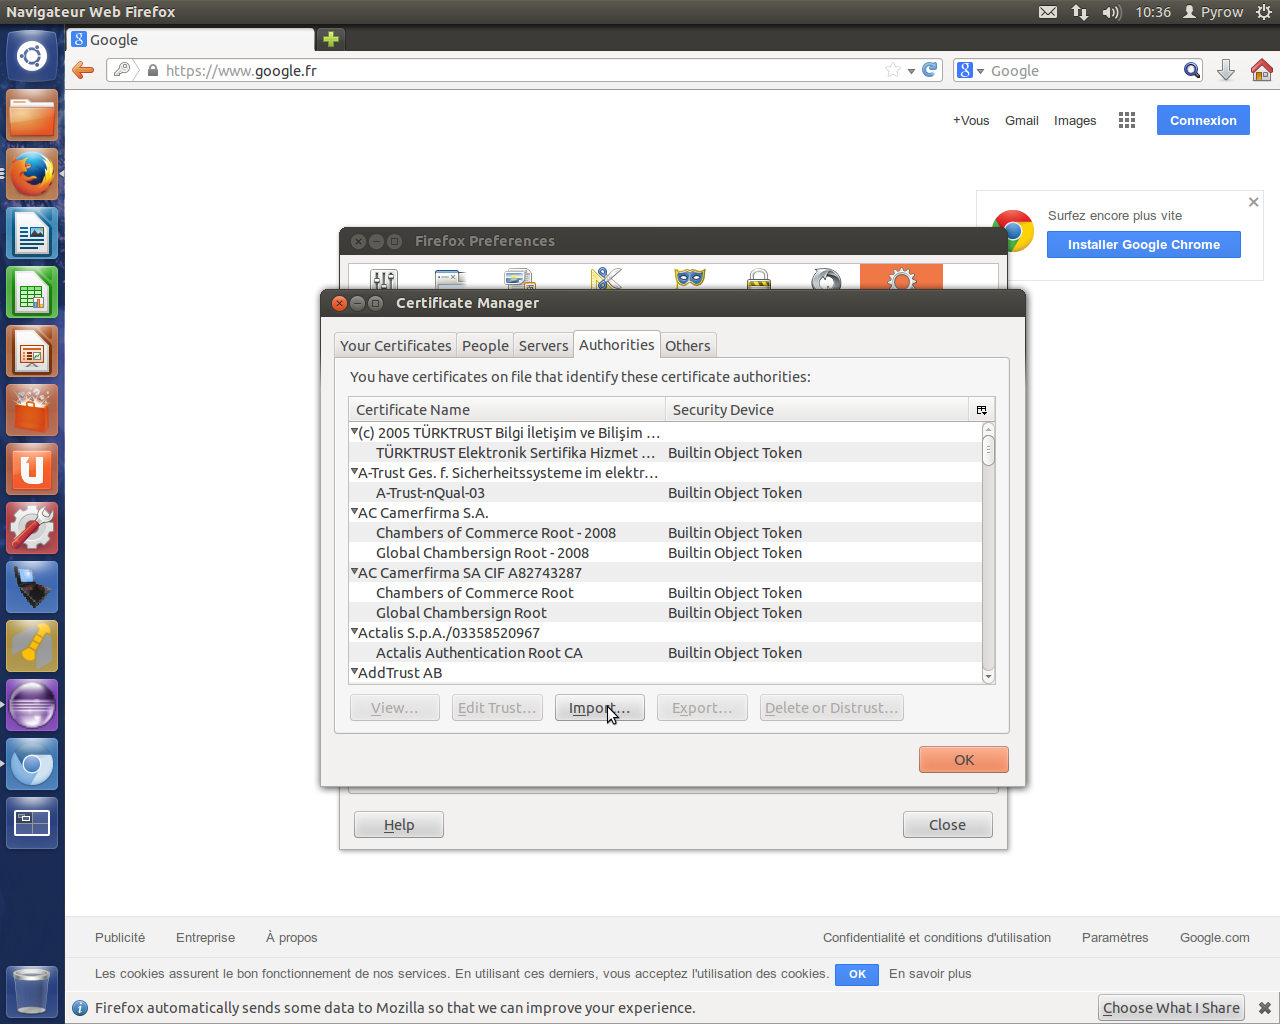
\includegraphics[width=\textwidth]{images/OngletCA.png}
\newpage
Il choisit ensuite le certificat de l'autorité qu'il veut installer puis valide.

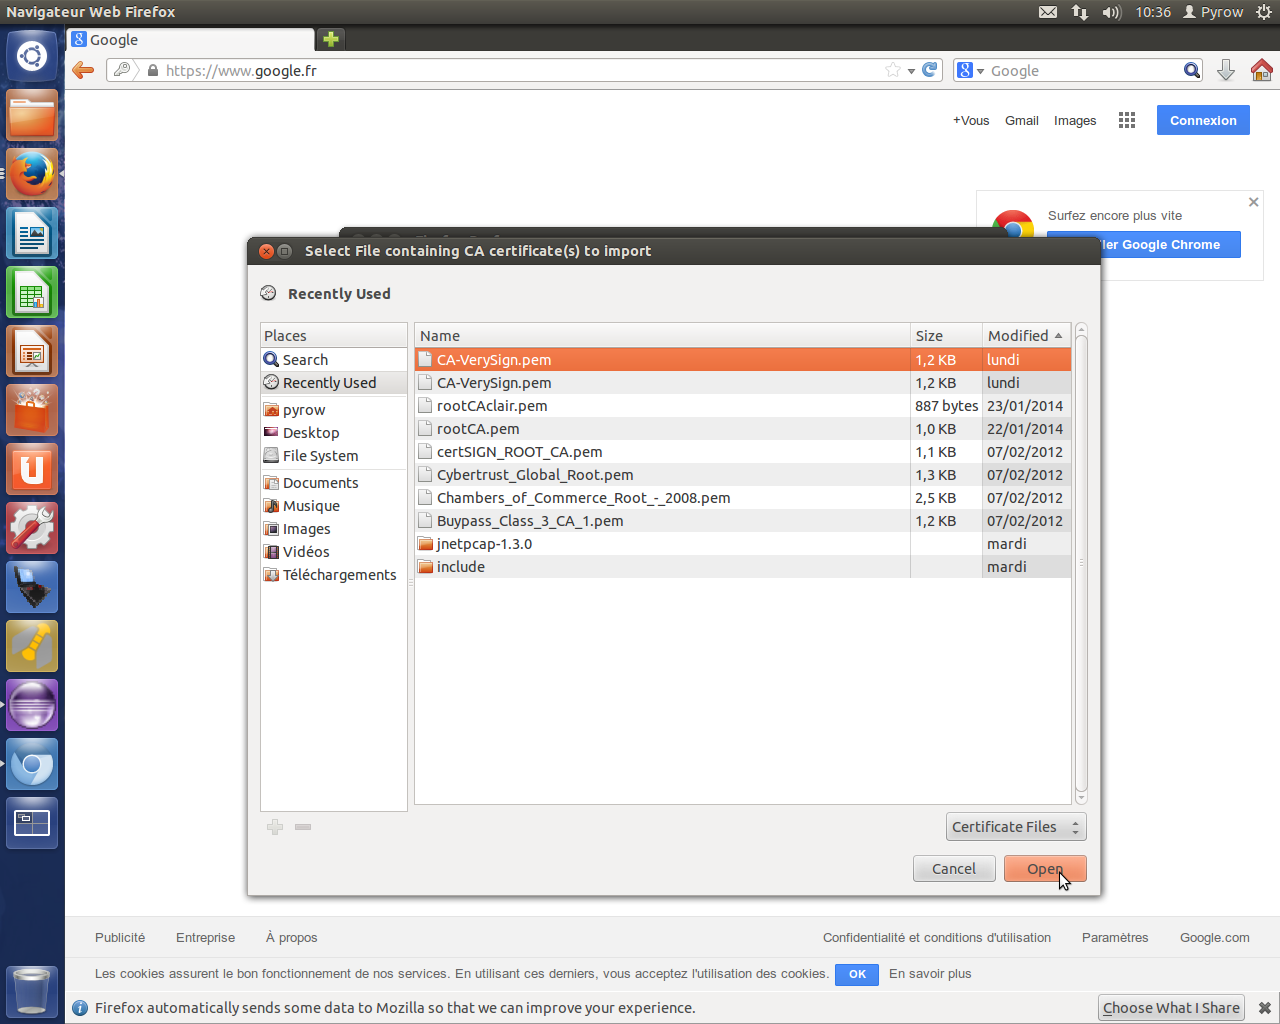
\includegraphics[width=\textwidth]{images/OngletImport.png}
\newpage
Une fenêtre s'ouvre et propose de faire confiance à cette autorité pour 3 types de Certificats. L'administrateur coche les 3 cases pour que son autorité soit reconnue valide sur tous les types puis clique sur ok.

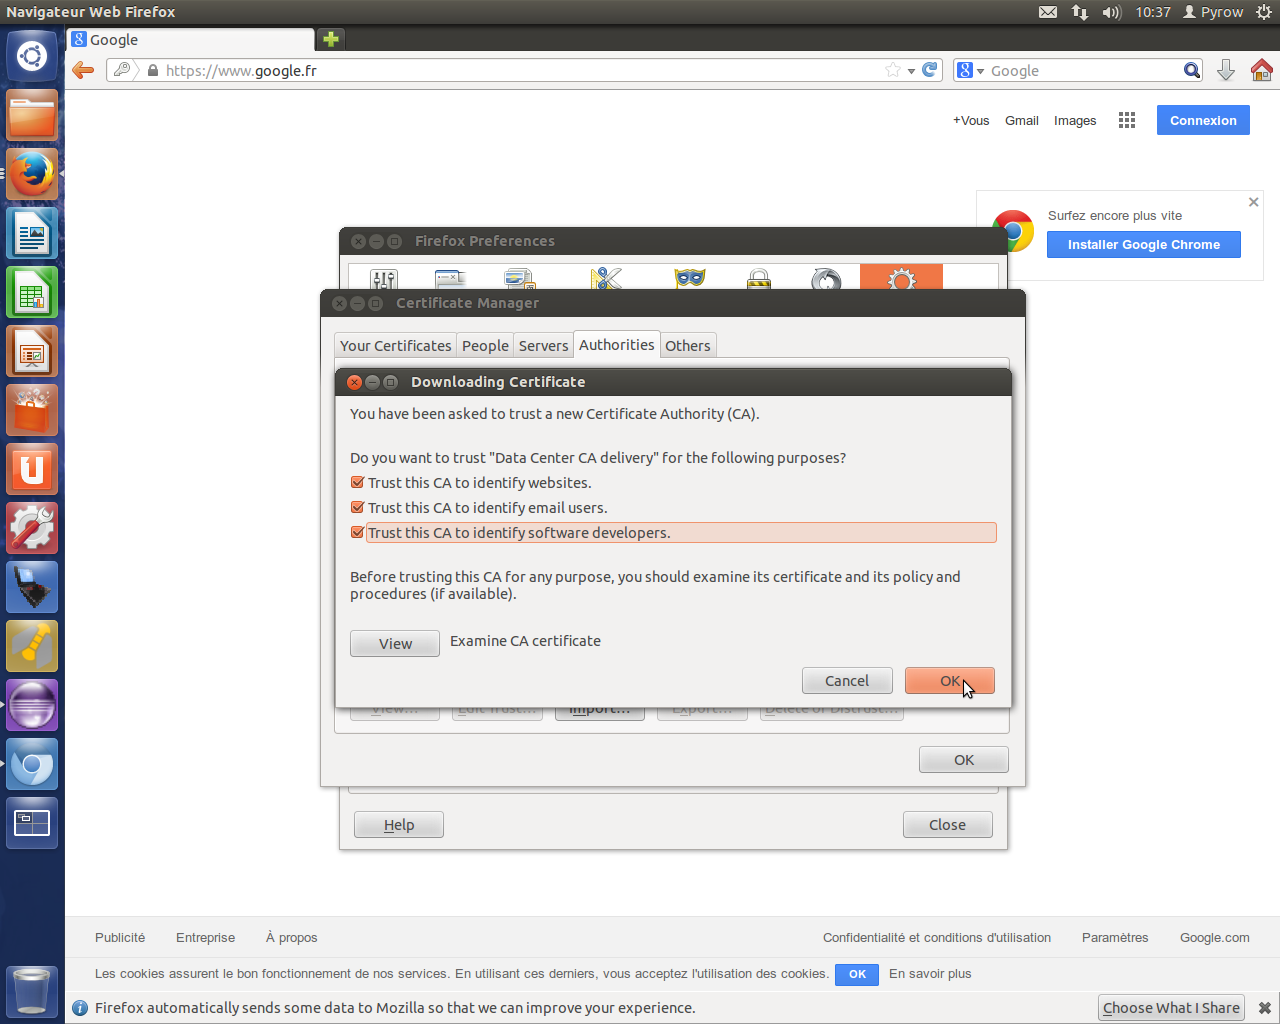
\includegraphics[width=\textwidth]{images/OngletConfirm.png} 


Voilà, l'autorité est installée et tous les certificats signés par cette autorité seront reconnus comme valides.
\newpage
\subsection{Chrome}

La démarche est très similaire à celle de firefox.

Tout d'abord, l'administrateur va dans Modifier > Préférences

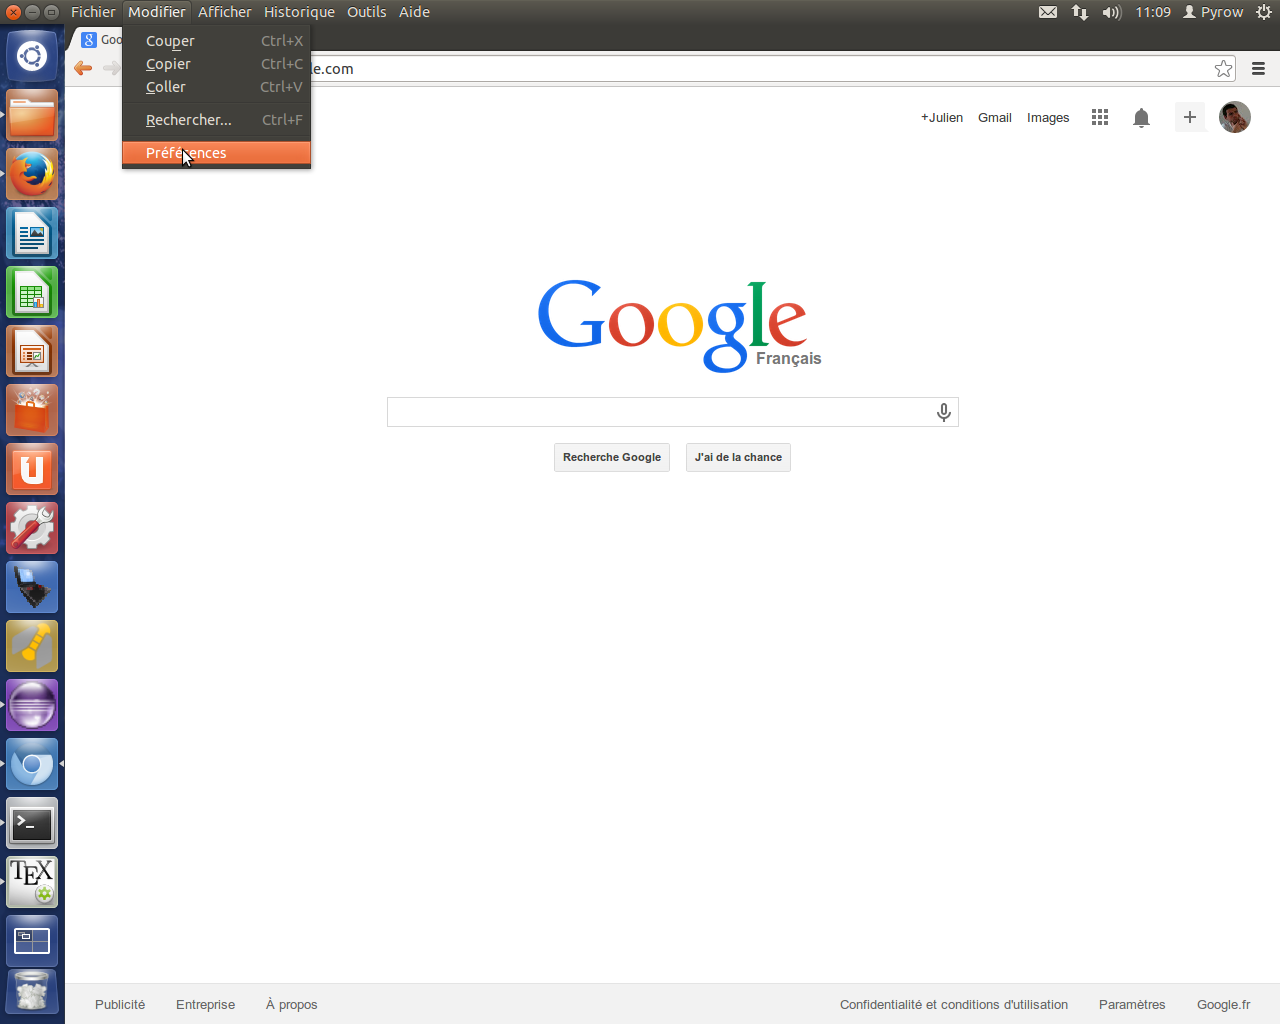
\includegraphics[width=\textwidth]{images/ChromePref.png} 
\newpage

Puis il clique sur Afficher les paramètres avancés.

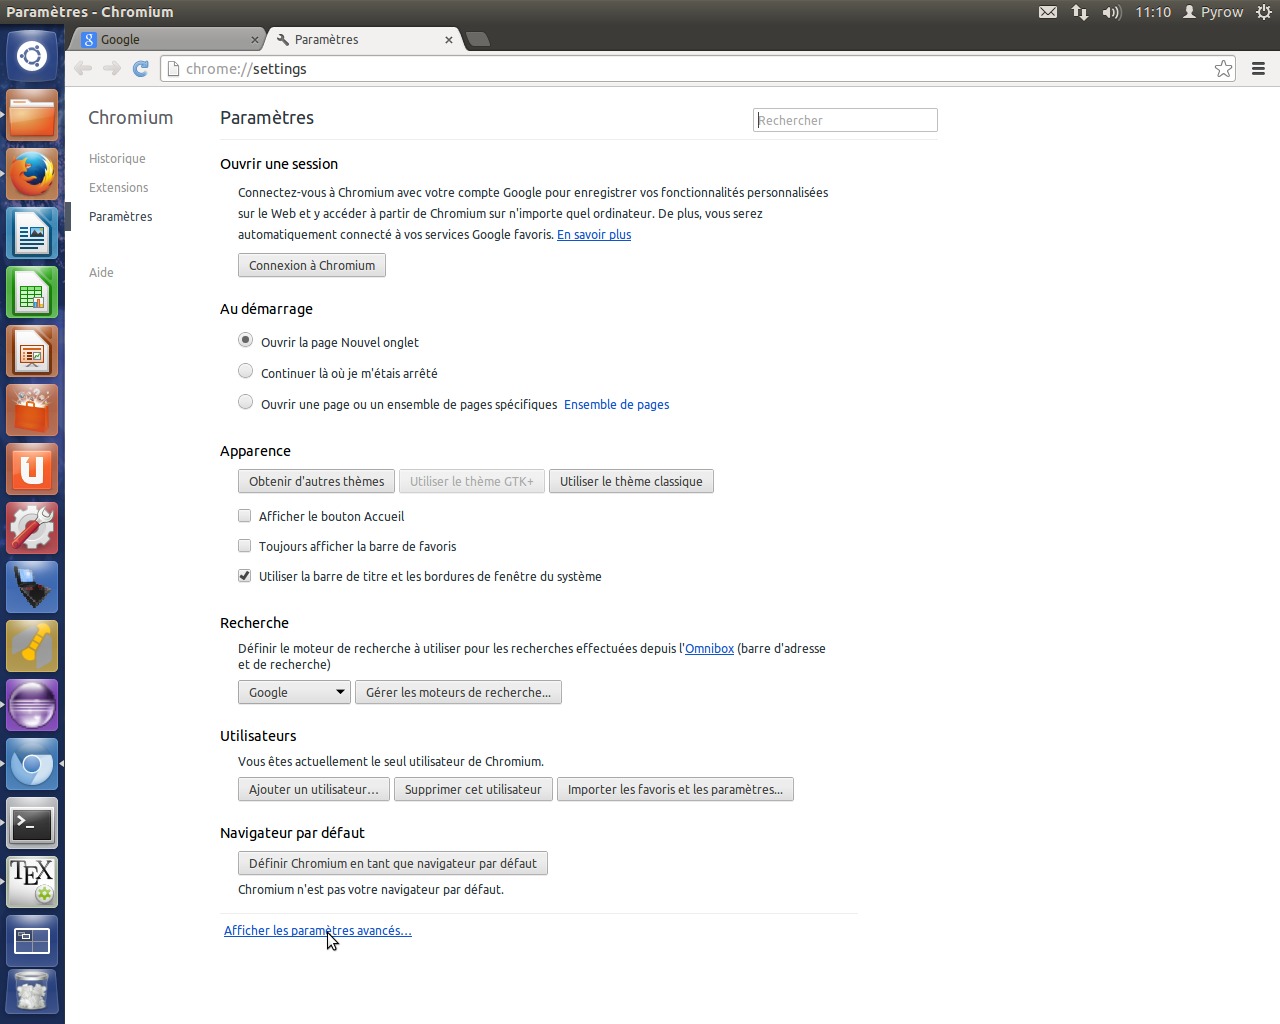
\includegraphics[width=\textwidth]{images/ChromeAvance.png} 
\newpage

Ensuite, dans la partie HTTPS/SSL, il clique sur Gérer les certificats

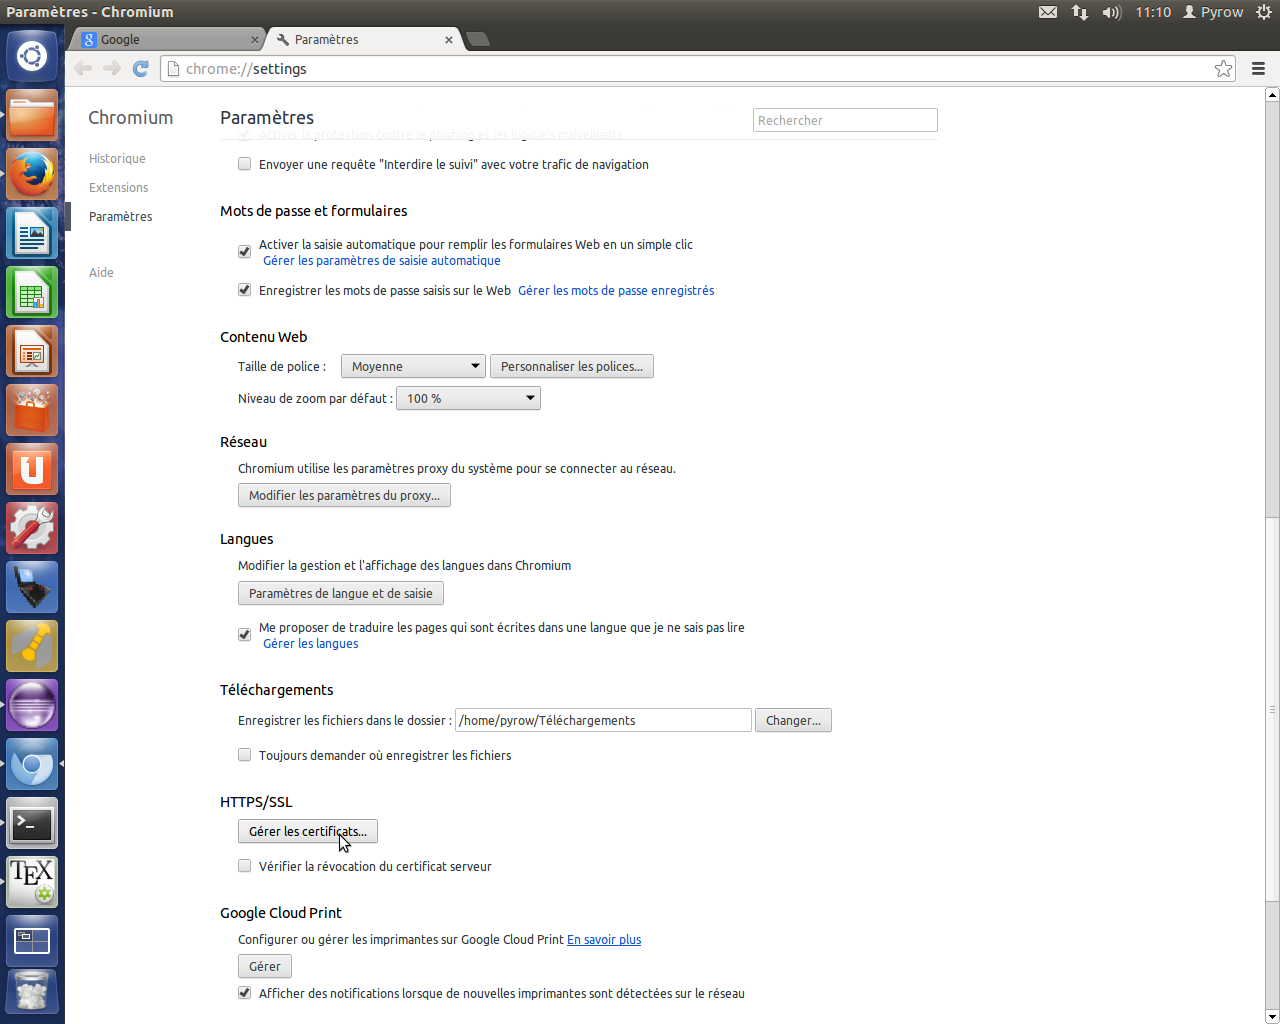
\includegraphics[width=\textwidth]{images/ChromeCert.png} 
\newpage

Il se déplace dans Autorités et clique sur Importer

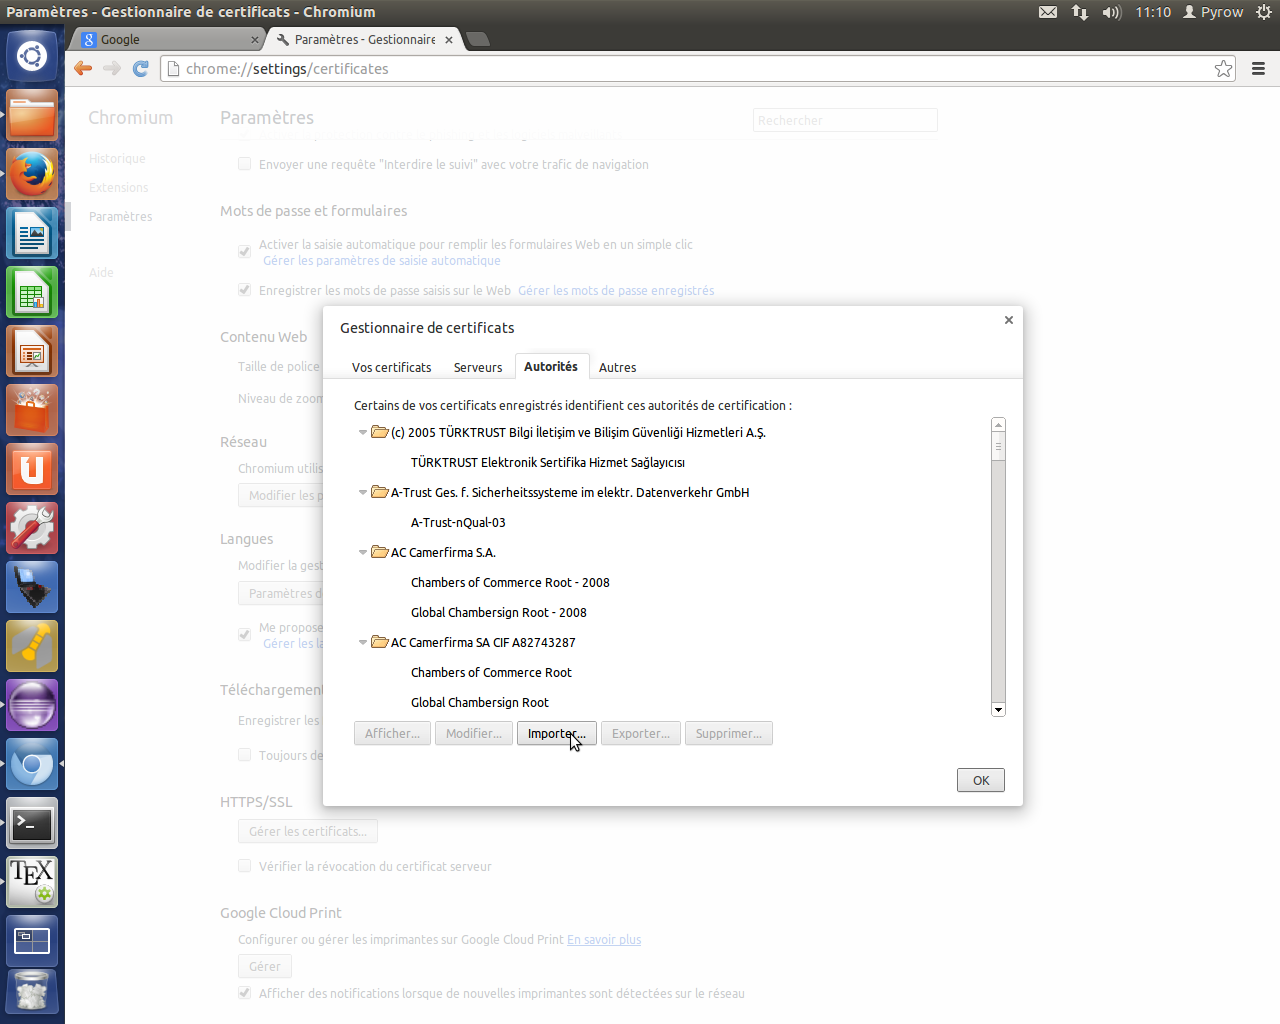
\includegraphics[width=\textwidth]{images/ChromeCA.png} 
\newpage

Il choisit le certificat de l'autorité et valide.

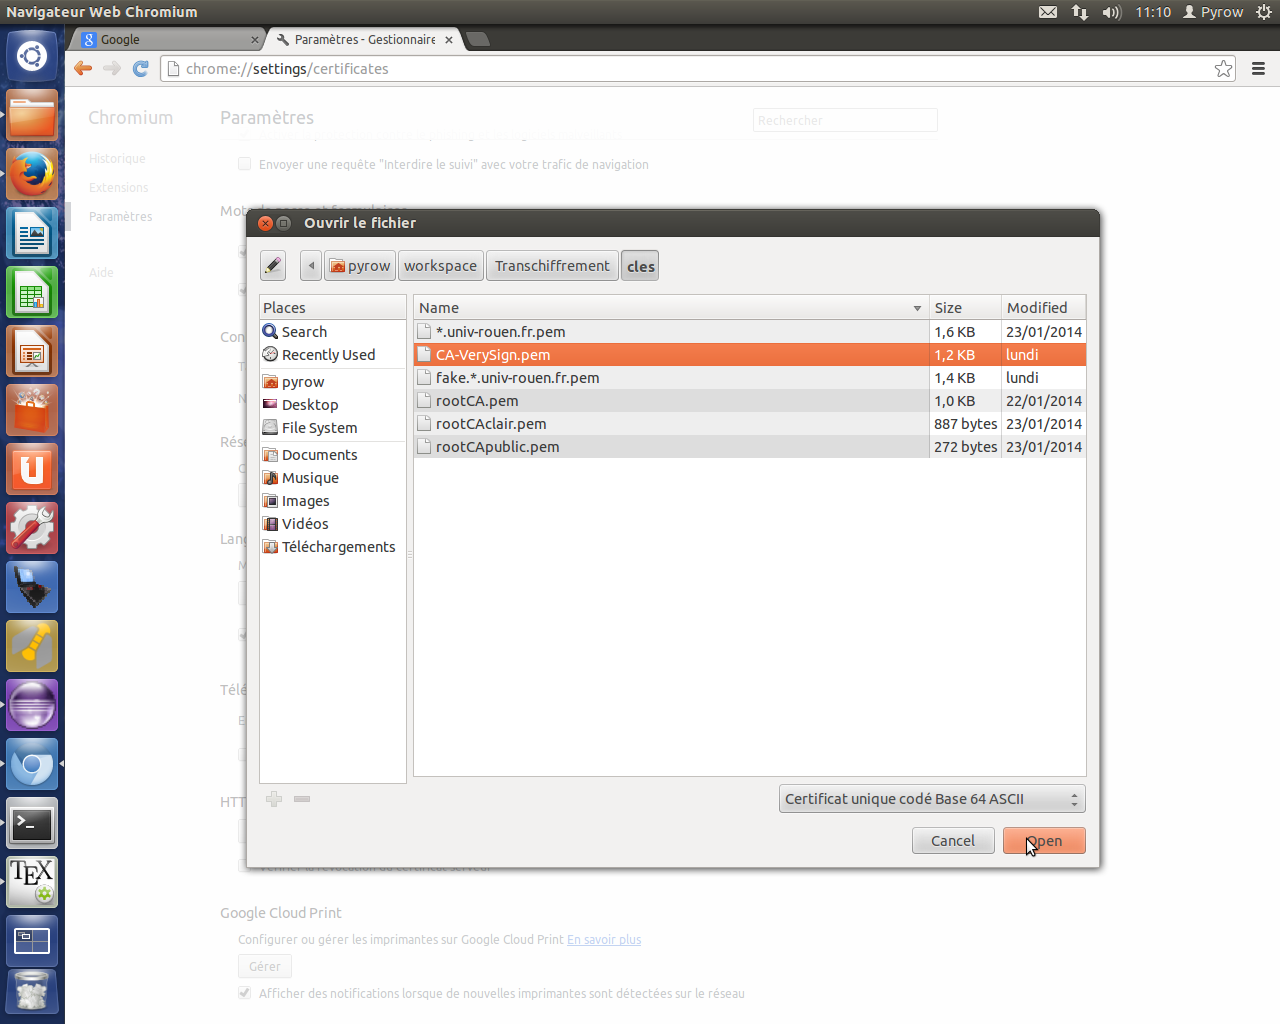
\includegraphics[width=\textwidth]{images/ChromeImport.png} 
\newpage

Enfin, il coche les 3 cases et clique sur ok pour finaliser l'installation de l'autorité.

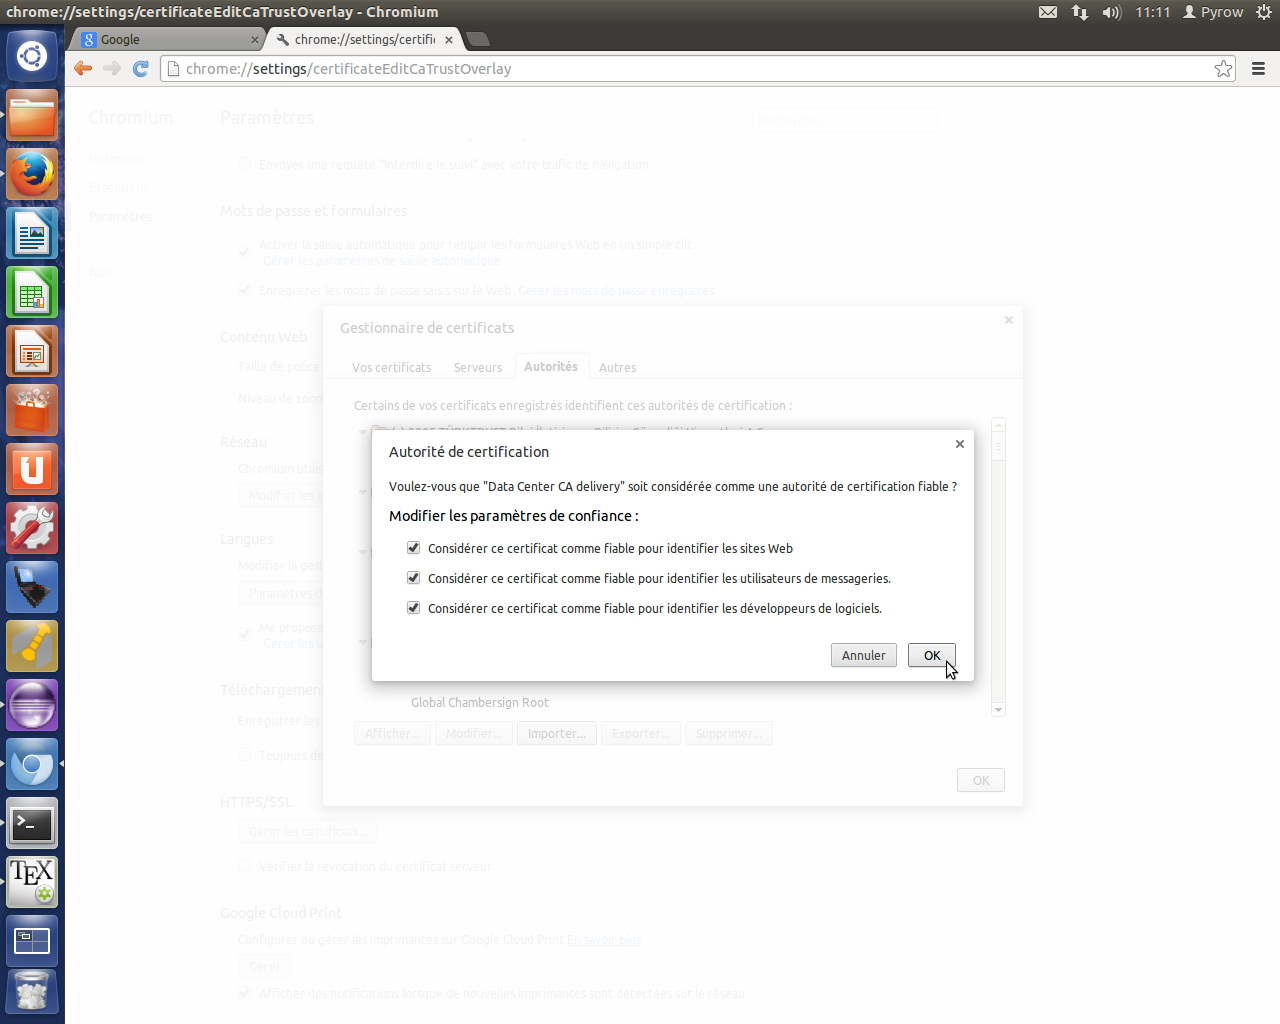
\includegraphics[width=\textwidth]{images/ChromeValide.png} 
\newpage

\section{Forcer l'acceptation de l'autorité par un client}
Dans cette section, nous forçons l'utilisateur a accepter notre autorité de certification. Si il ne l'a pas, il ne pourra pas naviguer sur internet.
Nous proposons donc un lien pour récupérer le certificat d'autorité sur lequel il faut cliquer.

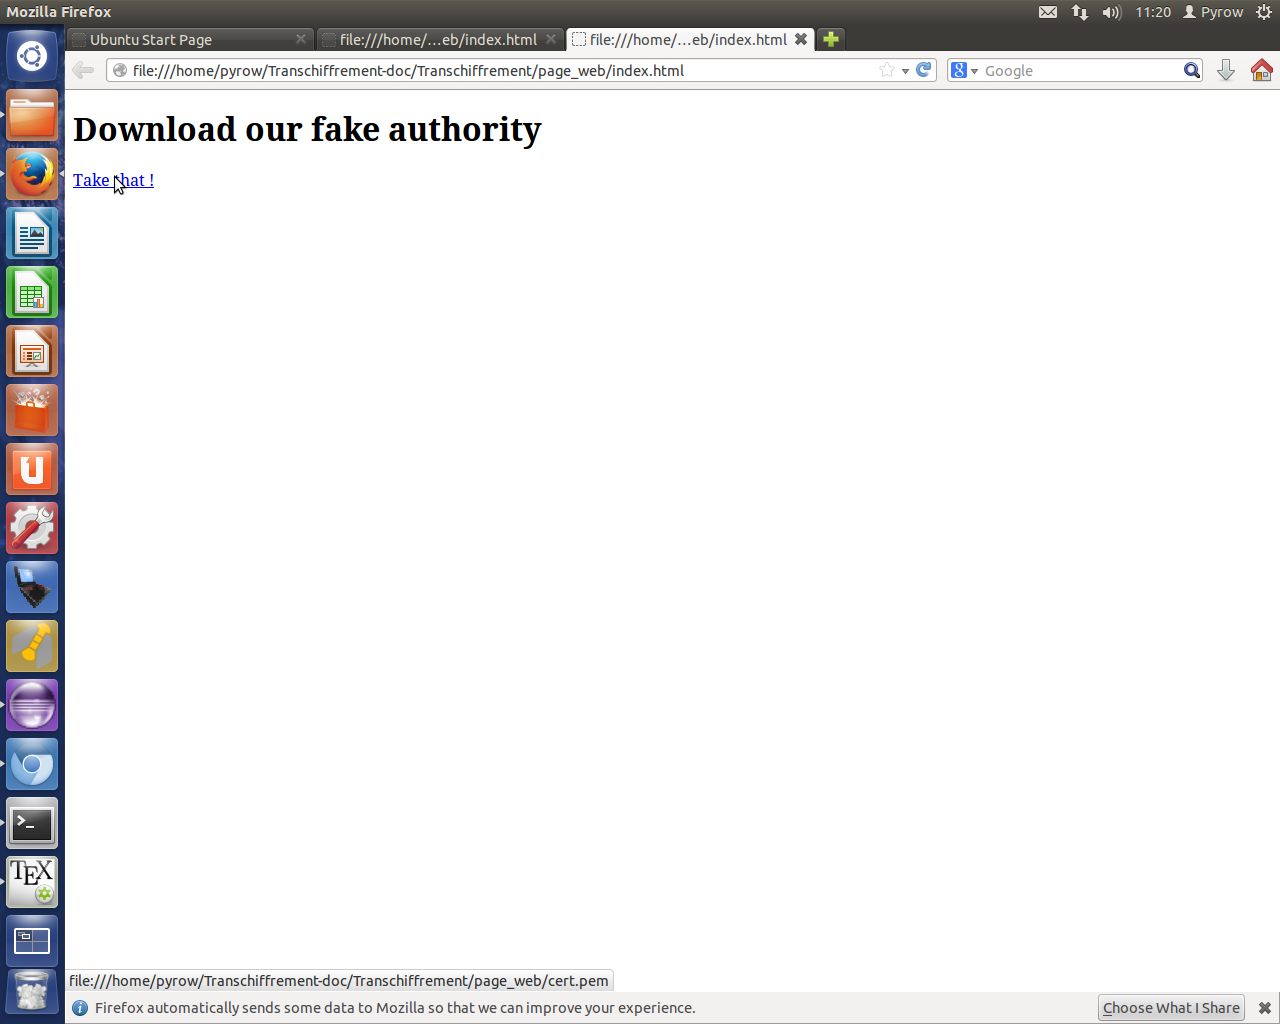
\includegraphics[width=\textwidth]{images/Page.png} 
\newpage

Ensuite, la fenêtre de validation s'ouvre et le client doit cocher les cases puis valider.

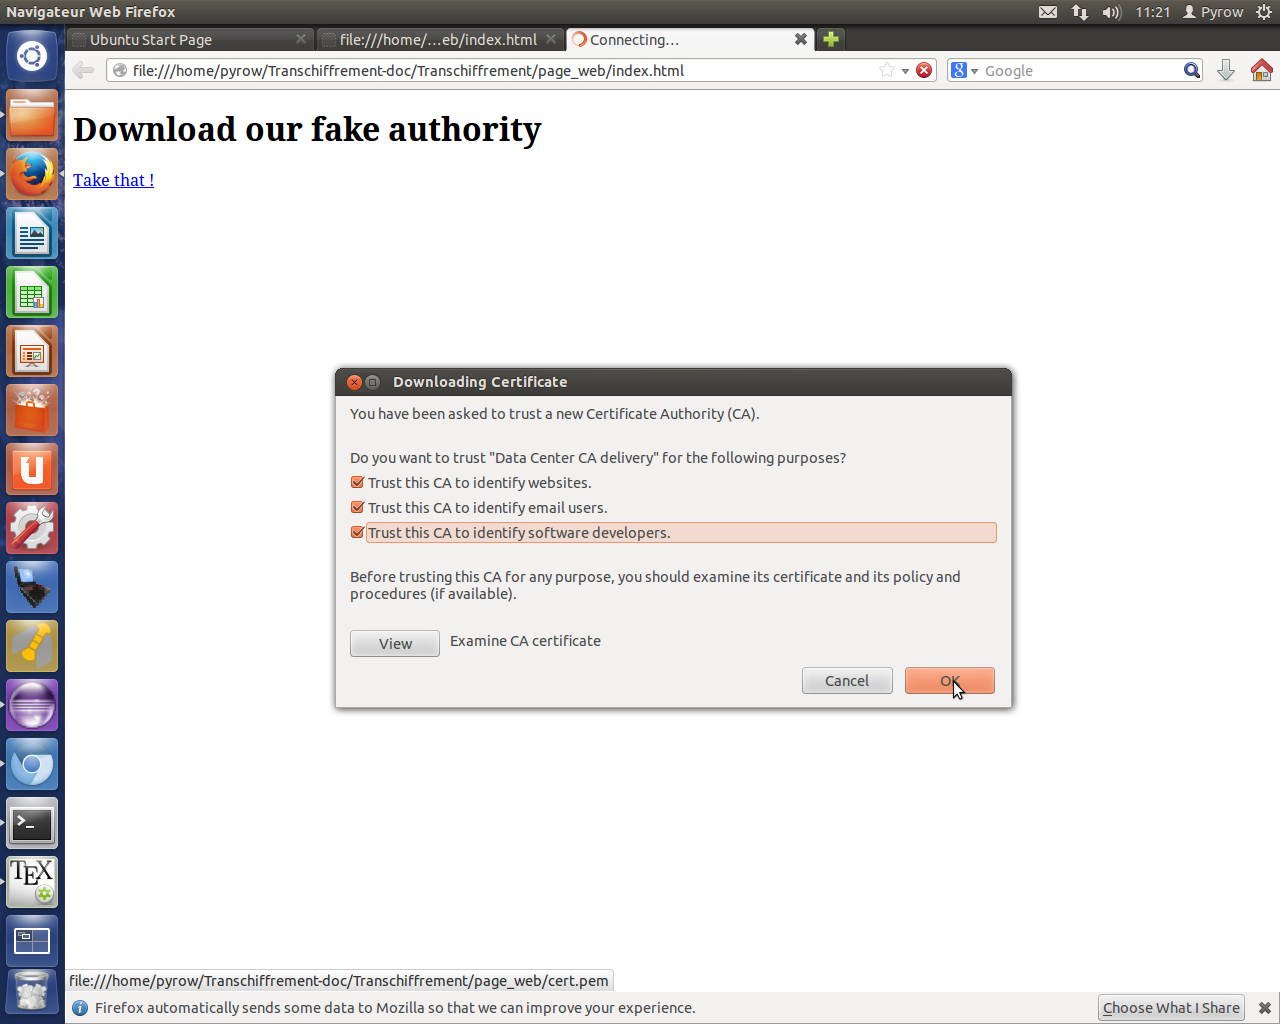
\includegraphics[width=\textwidth]{images/Cert.png} 
\newpage

A ce stade, l'autorité est installée et si le client veut retenter de l'installer, un message le prévient qu'il a déjà fini l'installation.

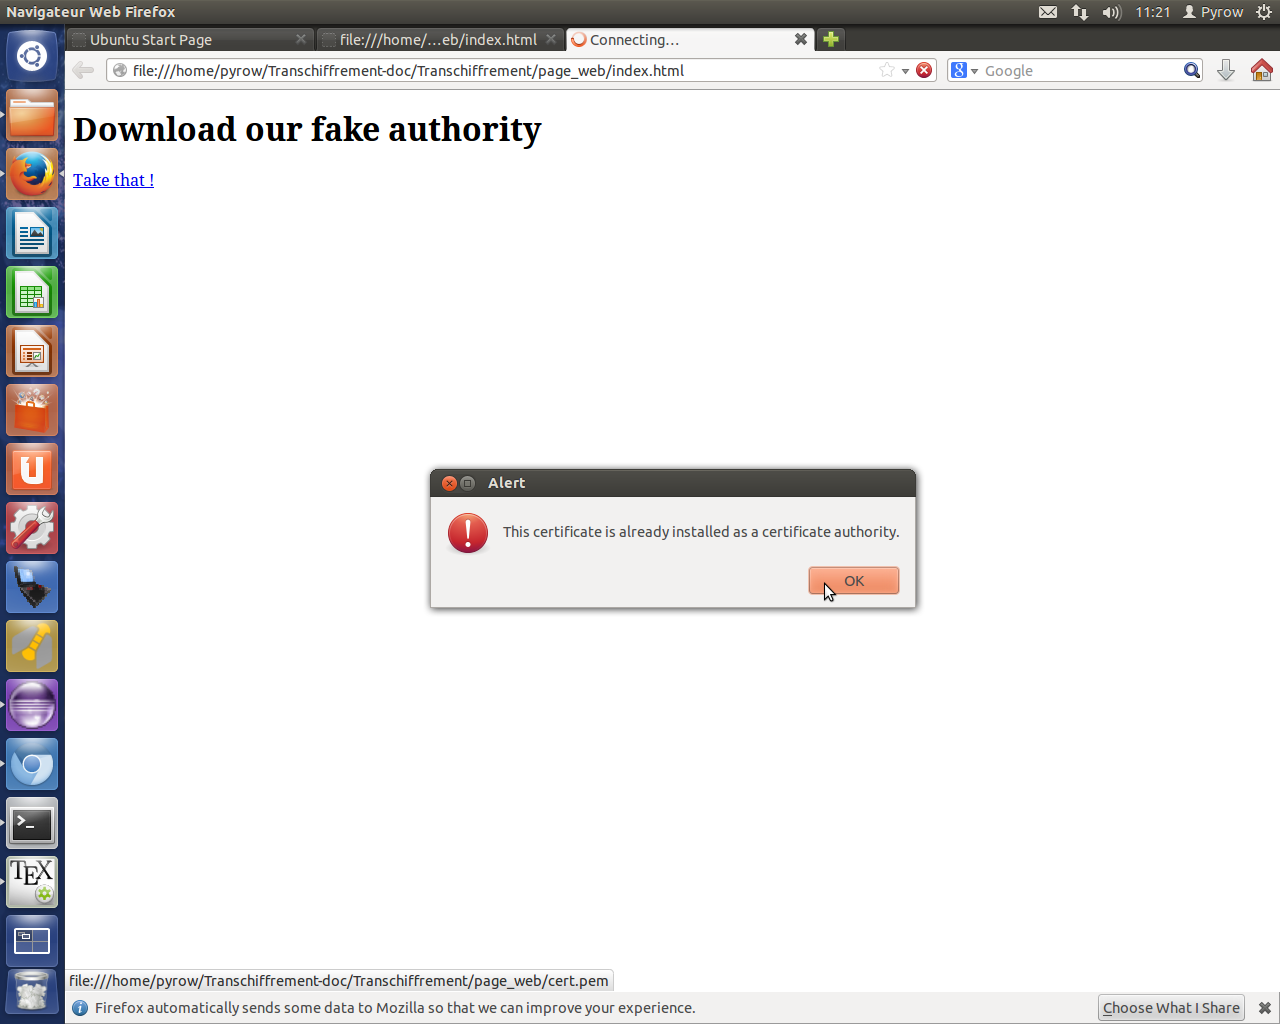
\includegraphics[width=\textwidth]{images/Alerte.png}

On peut voir qu'en seulement quelques clics, l'utilisateur installe une autorité dont il ne connaît rien et qui peut être utilisée pour déchiffrer toutes ses informations personnelles. 
\newpage
\end{document}